\documentclass[PICOAPC.tex]{subfiles}
\newcommand\pdeg{.\!\!\degree}
\newcommand\parcm{.\!\!'}


%\newpage
\section{Project Management, Schedule, and Cost}
\label{sec:project_management} %6

\subsection{Project Management Plan}
\label{sec:management_plan} %6.2

PICO benefits from the experience of predecessor missions such as \planck\ and \wmap, as well as many years of investment in technology development and a multitude of suborbital experiments. In addition to demonstrated science and engineering capabilities, this heritage has developed a community of people with the expertise required to field a successful mission.

This study assumes mission management by JPL with a Principal Investigator leading a single science team. A Project Manager provides project oversight for schedule, budget, and deliverables. A Project Systems Engineer leads systems engineering activities and serves as the Engineering Technical Authority. A Mission Assurance Manager serves as the Independent Technical Authority. The PICO mission development schedule is shown in Fig.~\ref{fig:Schedule}.

\begin{figure}[hb]
\begin{center}
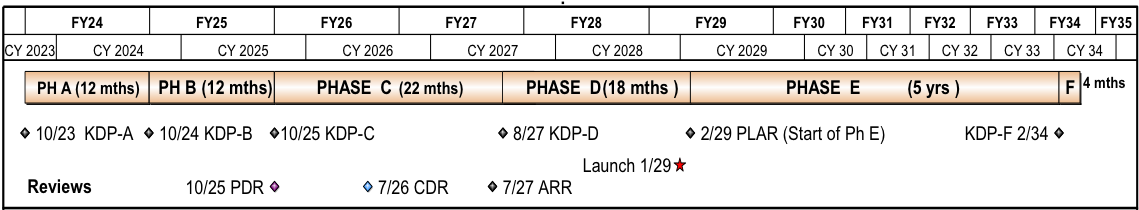
\includegraphics[width=\textwidth]{figures/Schedule.png}
\end{center}
\vspace{-0.25in}
\caption{\captiontext The PICO baseline schedule is based on historical actuals from similarly-sized missions such as Juno and SMAP. Per NASA direction, Probe studies assume a Phase~A start in October 2023.\label{fig:Schedule}}
\vspace{-0.05in}
\end{figure}

Probes are medium-class missions, similar in cost scope to NASA's
New Frontiers missions, which are Category~1 and Risk Classification A
or B, with Phase A--D costs capped at $\sim$ \$850M (not including the
launch vehicle). JPL is well-prepared to manage Probe missions, having
managed the Juno New Frontiers mission (launched 2011) and also the
development of the medium-class \textit{Spitzer} Space Telescope (launched
2003). JPL delivered the bolometric detectors for the \textit{Planck}
HFI instrument (launched 2009). Presently, JPL is managing NEOCam, a
Discovery class infrared space telescope.

The PICO spacecraft provider will be selected during mission formulation. Multiple organizations are capable of providing a spacecraft bus to meet PICO's requirements. Lockheed Martin contributed to the PICO concept study, leveraging their experience with New Frontiers missions Juno and OSIRIS-REx.
 
\subsection{Heritage}
\label{sec:heritage} %6.3

%The successful \textit{Planck} mission provides science heritage for PICO. 
The technical heritage for PICO traces to multiple missions. Because PICO observes in the mm/sub-mm regime, the surface accuracy requirement for the reflectors is relatively easy to meet. PICO's reflectors are similar to \planck 's, but somewhat larger ($270 \,\, {\rm cm} \times 205\,{\rm cm}$ primary versus $189\,{\rm cm} \times 155\,{\rm cm}$)~\citep{Gloesener2006}. \textit{Herschel} observed at shorter wavelengths that required higher surface accuracy and had a larger reflector ($350\, \,{\rm cm}$ diameter primary)~\citep{Toulemont2004}.

The heritage of the PICO detectors and readout electronics (which are described in \S\,\ref{sec:focal_plane}, \S\,\ref{sec:detector_readout}) is described in \S\,\ref{sec:technology_maturation}.

PICO's detectors are cooled by a cADR (\S\,\ref{sec:cadr}) with requirements that are within the capabilities of current ADRs developed by Goddard Space Flight Center. These systems have been applied to several JAXA missions, including \textit{Hitomi}~\citep{Shirron2016}. PICO's 4\,K cryocooler (\S\,\ref{sec:4kcooler}) is a direct extension of the JWST MIRI design~\citep{Durand2008,Rabb2013}. PICO benefits from a simpler and more reliable implementation of the J-T system than was required for MIRI, in that no deployment of cooling lines is required, and all flow valving is performed on the warm spacecraft. Cooling multiple independent points with a J-T loop has been demonstrated on \planck\ with the JPL-supplied 18\,K cooler~\citep{Planck2011}. Structures similar to PICO's V-groove radiator assembly (\S\,\ref{sec:radiative_cooling}) are a standard approach for passive cooling, and were first described more than thirty years ago~\citep{Bard1987}. We baselined a simple honeycomb material construction like that successfully flown by \planck~\citep{ESA2009,Planck2011}.

%PICO's 4.5\,m diameter V-groove assembly fits inside the launch vehicle fairing.

Most requirements on the PICO spacecraft are well within typical ranges and can be met with standard high heritage systems (\S\,\ref{sec:spacecraft}). PICO's spin architecture and data volume requirements are less typical, and are discussed below.

The spin system is less demanding than the successful SMAP spin system. The PICO spin rate is 1\,rpm, and the mission requires $\sim220$\,N\,m\,s of spin angular momentum cancellation (\S\,\ref{sec:attitude_determination}).
Only data and power lines pass across the spin interface between the spinning and non-spinning modules (Fig.~\ref{fig:ArchitectureBlockDiagram}). With SMAP, a 6-m instrument antenna is spun at 14.6\,rpm, and it requires  359\,N\,m\,s of spin angular momentum cancellation~\citep{Brown2016}. Data and power successfully pass across the spin interface. 

Though PICO's data volume is notable by current standards, it is already surpassed by missions in development. The mission produces 6.1\,Tb/day of raw data which is compressed to 1.5\,Tb/day (\S\,\ref{sec:detector_readout}). Data downlinks occur daily, but we baseline storage of 3\,days of (compressed) data to mitigate missed telecom passes. This requires 4.5\,Tb of onboard storage, in family with the 3.14\,Tb solid-state recorder currently in use by Landsat~8 and much smaller than the 12\,Tb flash memory planned for NISAR~\citep{Jasper2017}. The baseline 150\,Mb/s Ka-band data downlink is an existing DSN catalog service~\citep{DSN2015}. The baseline mission generates 2,200\,Tb of raw (uncompressed) data per year, less than the 6,800\,Tb/year currently returned by Landsat~8 and 9,300\,Tb/yr planned by NISAR~\citep{Jasper2017}.

\medskip
\subsection{Risk Assessment}
\label{sec:risk_assessment} %6.4

\subsubsection{Pre-Mission Risks}
\label{sec:premission_risks} %6.4.1

Technology development (\S\,\ref{sec:technology_maturation}) is performed prior to the beginning of mission development, and is outside of the mission cost (per NASA direction), so associated risks do not represent threats to the cost of mission development. Rather, these technology development risks affect the availability of components for the baseline mission. A technology-related mission descope is described in \S\,\ref{sec:technology_descopes}.

\subsubsection{Development Risks}
\label{sec:development_risks} %6.4.2

PICO's healthy contingencies, margins, and reserves provide
flexibility to address risks realized during mission development. PICO
carries $>40\,\%$ instrument sensitivity margin (Table~\ref{tab:bands}),
$>100\,\%$ heat lift margin (Table~\ref{tab:cooler}), $43\,\%$ system
power contingency, $31\,\%$ payload mass contingency, and $25\,\%$
spacecraft mass contingency. The Falcon~9 launch capability (assuming ocean
recovery) exceeds PICO's total launch mass (including contingency) by
a $50\,\%$ margin. The PICO budget includes $30\,\%$ cost
reserves for Phases A--D (\S\,\ref{sec:mission_cost}).

%During mission development the Project Systems Engineer continually assesses risks, tracks progress toward retiring them, and updates mitigations. 
Mitigations for %a few top
the risks identified during this study are described below. \\
$\bullet$ \hspace{0.05in} Thermal risk can be mitigated through extensive thermal modeling and
review in Phase A, and design for early test verification. \\
$\bullet$ \hspace{0.05in} Risks associated with the instrument spin architecture can be mitigated by engaging JPL engineers who were involved in the SMAP mission. \\
$\bullet$ \hspace{0.05in} Detector delivery schedule risk can be mitigated by beginning fabrication early in the project life cycle and fabricating a generous number of detector wafers to ensure adequate yield. Multiple institutions (including, for example, JPL, GSFC, NIST, and ANL) would be capable of producing the PICO detectors. \\
%Suborbital programs generally achieve $>66\,\%$ detector wafer yield. \\
$\bullet$ \hspace{0.05in} Risks associated with the integration and test of a cryogenic instrument can be mitigated through advanced planning and allocation of appropriate schedule and schedule margin.

\subsubsection{Operations Risks}
\label{sec:operations_risks} %6.4.3
\input tables/table6.1_wrap.tex 

The PICO design meets the requirements associated with the NASA Class~B risk classification. For Class~B missions, essential spacecraft and instrument functions are typically fully redundant. This increases mission cost, but significantly reduces the risk of mission failure.

The PICO mission utilizes a single instrument with a single observing mode mapping the sky using a repetitive survey pattern. The mission does not require any time-critical activities. The observatory fits into 
the launch vehicle fairing in its operational configuration, therefore no hardware deployments are required. 
Because PICO observes at long wavelengths, the telescope does not require a dust cover (nor the %associated
 mission-critical cover release).

The spacecraft incorporates a fault protection system for anomaly
detection and resolution. The Sun-pointed, command receptive,
thermally stable safe-mode attitude allows ground intervention for
fault resolution without time constraints. PICO's high degree of
hardware redundancy and onboard fault protection ensure spacecraft
safety in the event of unforeseen failures and faults.

As described in \S\,\ref{sec:signal_separation} and
\S\,\ref{sec:systematics}, pre-Phase A simulation software maturation
is recommended to mitigate the challenges associated with foreground
separation and systematics control.

%\newpage  % temporay newpage to make wrapfig work and allow better length estimate of document.  to be removed!!

\medskip
\subsection{Mission Cost}
\label{sec:mission_cost} %6.5
%\costfootnote
%
%\input tables/table6.1-2_vert_wrap.tex

We estimate PICO's total Phase A--E lifecycle cost between \$870M and \$960M, including the \$150M allocation for the Launch Vehicle (per NASA direction). These cost estimates include 30\,\% reserves for development (Phases A--D) and 13\,\% reserves for operations (Phase~E). Pre-Phase-A technology maturation 
%(\S\,\ref{sec:technology_maturation}) 
will be accomplished through the normal APRA and SAT processes, and is not included in the mission cost. 
%(per NASA direction).

Table~\ref{tab:cost} shows the mission cost breakdown, including the JPL Team~X\cref{teamx} cost estimate, as well as the PICO team cost estimate. Team~X estimates are generally model-based, and were generated after a series of instrument and mission-level studies. Their accuracy is commensurate with the level of understanding typical to Pre-Phase-A concept development. They do not constitute an implementation or cost commitment on the part of JPL or Caltech.

The PICO team has adopted the Team~X estimates, but also obtained a parametrically estimated cost range for the Flight System (WBS 6) and Assembly, Test, and Launch Operations (ATLO, WBS~7) from Lockheed Martin Corporation to represent the cost benefits that might be realized by working with an industry partner. After adding estimated JPL overhead and Team~X estimated V-groove assembly costs (not included in the Lockheed estimate), the PICO team cost is in-family with but lower than the Team~X cost.

Management, Systems Engineering, and Mission Assurance (WBS 1--3)
development costs scale linearly with the WBS 4--12 development costs
in the Team~X model, and are adjusted accordingly in the PICO team
estimate. Science team (WBS~4) costs are assessed by Team~X based on PICO
science team estimates of the numbers and types of contributors and
meetings required for each year of PICO mission development and
operations. These workforce estimates are informed by recent
experience with the \textit{Planck} mission.

Payload system (WBS~5) costs are discussed in detail in
\S\,\ref{sec:instrument_cost}.  PICO's spacecraft (WBS~6) cost
reflects a robust Class~B architecture
(\S\,\ref{sec:spacecraft}). Mission-critical elements are
redundant. Appropriate flight spares, engineering models and
prototypes are budgeted. The V-groove assembly (\S\,\ref{sec:radiative_cooling})
is costed in WBS~6.  Mission operations (WBS~7), Ground Data Systems
(WBS~9), and Mission Navigation and Design (WBS~12) costs reflect a
relatively simple concept of operations (\S\,\ref{sec:operations}). PICO has a single
instrument and a single science observing mode. It surveys the sky
continuously using a pre-planned repetitive survey pattern. Orbit
maintenance activities are simple and infrequent.

\subsubsection{Payload Cost}
\label{sec:instrument_cost} %6.5.1

\input tables/table6.2_wrap.tex

The PICO payload consists of a single instrument: an imaging
polarimeter. Payload costs are tabulated in
Table~\ref{tab:instrument_cost}.

The superconducting detectors require sub-kelvin cooling to
operate. The active cooling system (the 0.1\,K cADR and 4\,K
cryocooler, \S\,\ref{sec:cadr} and \S\,\ref{sec:4kcooler}) comprises nearly half of the payload
cost. The cADR cost for this study is an estimate from Goddard
Space Flight Center, and assumes the provision of both a flight
model and an engineering model. GSFC has produced ADRs for multiple
spaceflight missions. The 4\,K cryocooler cost for this study is based
on the NASA Instrument Cost Model (NICM) VIII CER Cryocooler model
\cite{Mrozinski2017}, assuming a commercial build. PICO benefits
greatly from recent and ongoing investment by commercial suppliers of
4\,K coolers (as described in \S\,\ref{sec:4kcooler}).  Team~X used NICM~VIII to model
the cost of the focal plane and dual string readout electronics (\S\,\ref{sec:focal_plane},
\S\,\ref{sec:detector_readout}).  Team~X estimated the telescope cost using the Stahl model
\cite{Stahl2016}. The telescope is not a major cost driver, primarily
because the reflectors only need to be diffraction limited at 330\,$\mu$m
(900\,GHz) (\S\,\ref{sec:telescope}).

Based on JPL experience, 18\,\% of the instrument cost is allocated for integration and testing (I\&T). This includes I\&T of the flight focal-plane assembly with the flight cADR and then I\&T of the complete instrument including the focal-plane assembly, reflectors, structures, and coolers (\S\,\ref{sec:iandt}). I\&T of the instrument with the spacecraft is costed in WBS~10 (ATLO).
%\costfootnote

%\newpage

% [Amy] NASA recently dictated that all Probes add a cost table using
% their standard template. This does not count against the 50 page
% limit. We should paste this in as a graphic rather than converting
% it to a LaTeX table – the whole idea is to standardize, so
% reformatting is not appropriate. The existing cost section (6.5)
% remains (including Table 6.1) – this is an add-on, and should get
% its own page.

%\section*{NASA Standard Template Cost Table}

%\begin{centering}
%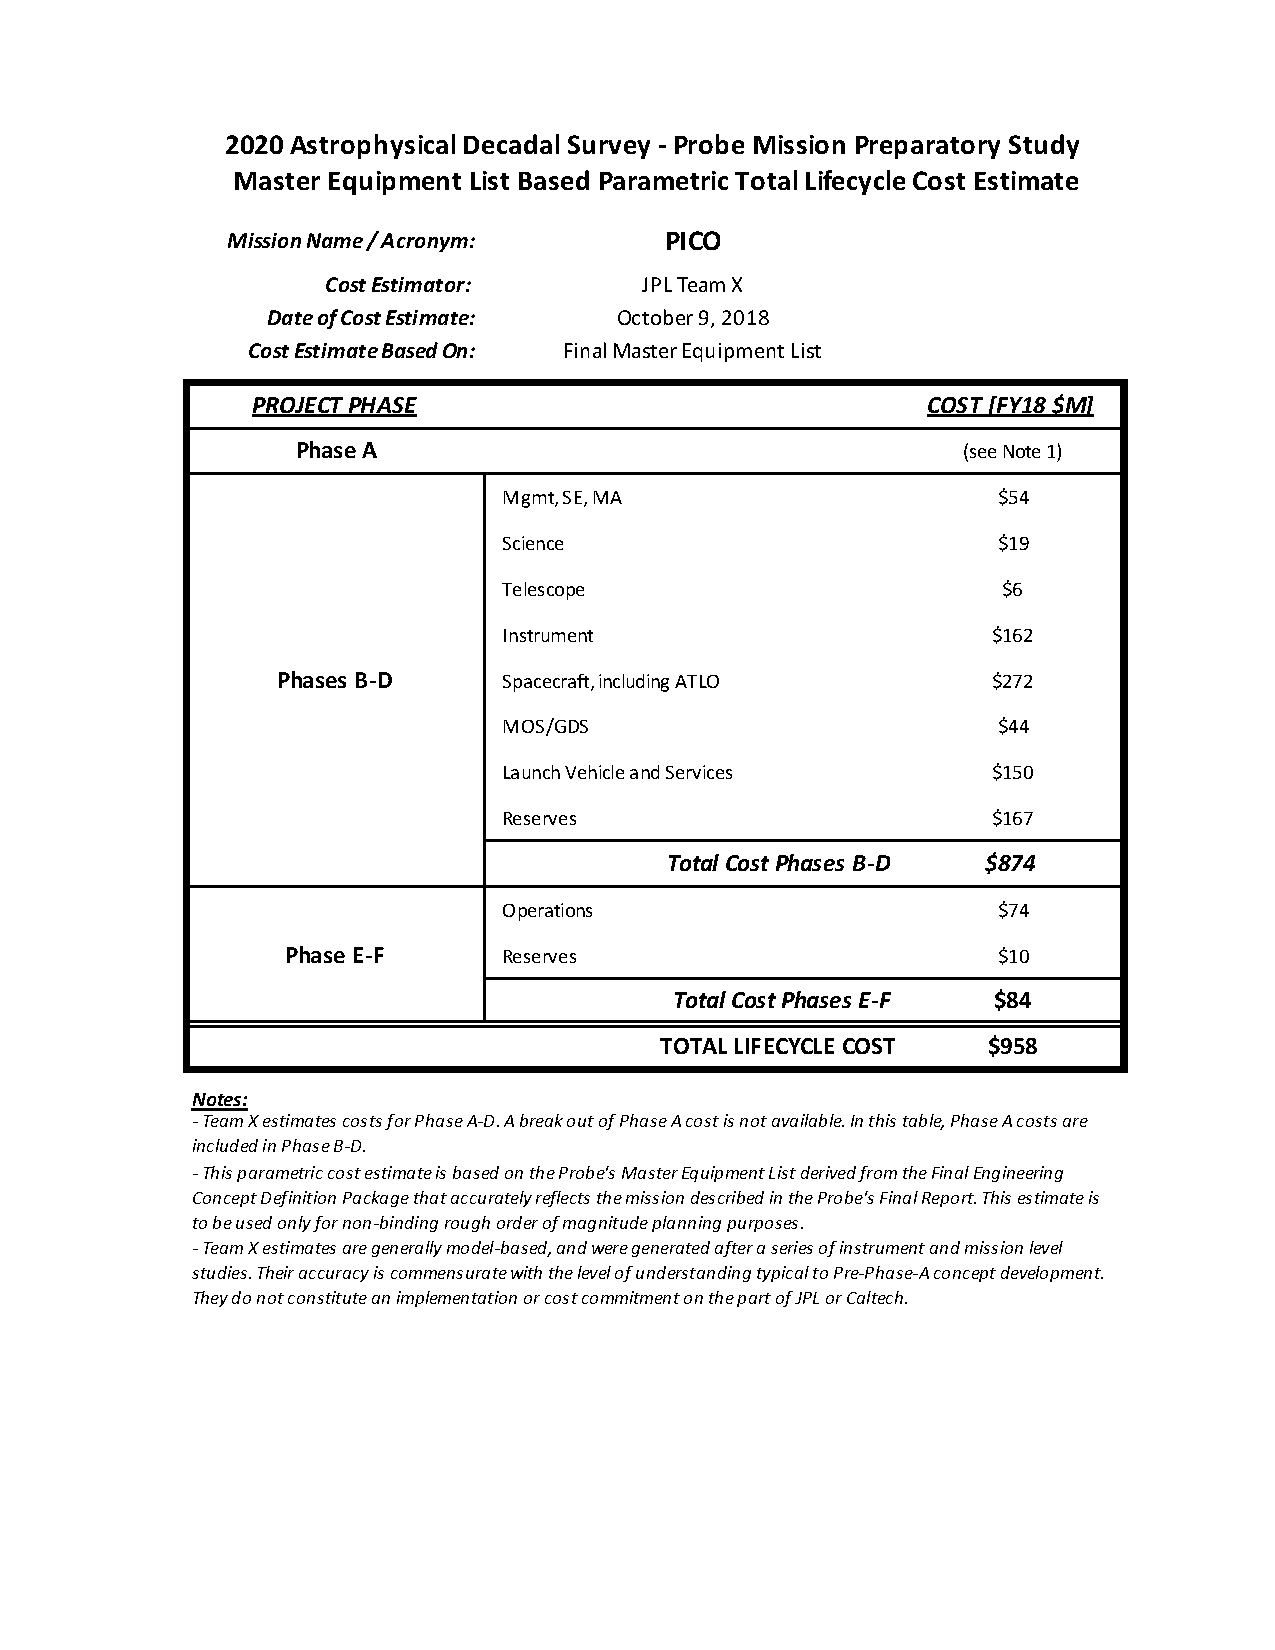
\includegraphics{tables/PICO_Standard_Cost_Table.pdf}
%\end{centering}
